\documentclass[letterpaper,12pt]{article}
\usepackage[utf8]{inputenc}
\usepackage{fullpage}
\usepackage{courier}
\usepackage[margin=0.75in]{geometry}
\usepackage{listings}
\usepackage{color}
\usepackage{graphicx}
\usepackage[width=5in]{caption}
\usepackage{hyphenat}
\usepackage[section]{placeins}
\usepackage{cmll}
\usepackage{float}
\usepackage{hyperref}

% Format a sectionless paragraph
\newcommand*\unparagraph{
	\par
	\nopagebreak
	\vskip3.25ex plus1ex minus.2ex
	\noindent
}

% define extra colors
\definecolor{dkgreen}{rgb}{0,0.6,0}
\definecolor{purple}{RGB}{159,0,197}

% define the code listing format
\lstset{
	language=C++,
	basicstyle=\footnotesize\ttfamily,
	backgroundcolor=\color{white},
	showspaces=false,
	showstringspaces=false,
	frame=none,
	tabsize=3,
	keywordstyle=\color{purple},
	commentstyle=\color{dkgreen},
	stringstyle=\color{blue},
	escapeinside={\%*}{*)}
}

% define the title/header
\title{\Large CS 1428 Honors\\Lab 6}
\author{Jared Wallace}
\date{}

\begin{document}

\maketitle

\vspace{30mm}

\section*{Conway's Game of Life}
Conway's Game of Life is an attempt to model real life through a simplified representation.
As such, it can be described as a "life" simulator. In this simulator, there exist two states;
alive and dead. Each person is represented by a cell. Any given cell, at any given time, is either
dead or alive. When started, the simulator proceeds through iterations, or generations. Each time
the game iterates, cells change states or stay the same based on a few simple rules.
The simulation is what's known as a \emph{zero player game}, which means that once you start the
simulation, it proceeds without any further input from the user.
More information is available on Wikipedia if needed.

\section*{Our implementation}
We will be implementing a basic version of the Game of Life. We will use a two-dimensional array as
our "world", with each element representing a cell in the game. Our two states will be represented as
blank(dead), and an asterisk(alive). When the program iterates the world, each cell will change state
based on the number of living neighbors it has. The rules that determine what happens are as follows:
\begin{table}[H]
\begin{center}
    \begin{tabular}{|c|c|c|}
        \hline
        \textbf{Living Neighbors} & \textbf{Currently Alive} & \textbf{Currently Dead} \\ \hline
        Fewer than 2 & Dies & Stays Dead \\ \hline
        2 & Stays Alive & Stays Dead \\ \hline
        3 & Stays Alive & Becomes Alive \\ \hline
        Greater than 3 & Dies & Stays Dead \\ \hline
    \end{tabular}
\end{center}
\end{table}

The requirements for your program are as follows:
\begin{itemize}
    \item Must process at least 10 iterations, or generations
    \item Must display each generation in turn, along with a label indicating the generation number
\end{itemize}

Hint: Keep in mind that you will need to write the next generation to a \emph{seperate} two-dimensional
array in order to avoid corrupting the current game board, and then copy the new generation to the array 
that is displayed.

I have also provided some starter code to assist you (starter.cpp).
\section*{Deliverables}
Hard copy of the source code you wrote (lab6h.cpp). Soft copy (upload to homework upload) of
your source code.

% Comic at the bottom
\begin{figure}[ht!]
	\centering
	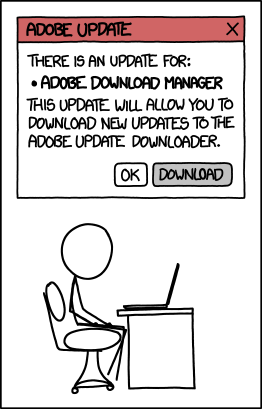
\includegraphics[width=3in]{all_adobe_updates.png}
    \caption*{ALERT: Some pending mandatory software updates require version 21.1.2 of the Oracle/Sun Java(tm) JDK(tm) Update Manager Runtime Environment Meta-Updater, which is not available for your platform.}
\end{figure}
\end{document}
